\section{Motivation}
\begin{frame}[t]{Motivation}
    \vspace{0.5cm}
	\only<1->{
        \begin{itemize}
    		\item NP phenomenology depends on free parameters \\
            {\footnotesize And usually more than we'd like!}\\
            {\footnotesize E.g. points in the space of Wilson coefficients}
    		\item NP influences shape of kinematic distributions
    	\end{itemize} 
    }
	
	\only<2->{
        \bigskip
    	\stress{Problems:}
    	\begin{itemize}
            \item {\color{purple}Theorist}: parameters $\lra$ predict kinematic distribution \\
            {\footnotesize Also important for experimentalists: Are we sensitive to anything interesting?}
    		\item {\color{purple}Experimentalist}: measured kinematic distribution $\lra$ exclusion limits
        \end{itemize}
        \smallskip
        \stress{BUT}: How to present results? {\footnotesize There are no nice ways to visualize 3+ dimensions!}
    }
    
    \only<3->{
        \bigskip
        \stress{Even worse}:\\
        
        {\color{purple}Experimentalists} need to make \stress{assumptions} on kinematic distribution for their measurements!
    }
\end{frame}
%
\begin{frame}[t]{Motivation II}{Example}
	\mauthor{BaBar}'s result for $R(D^{(*)})=\frac{\,\bddstaunu}{\bddsellnu}$ based on model assumption\\
	{\footnotesize(2HDM with specific $\tan\beta$ parameter -- \mauthor{1205.5442})}\\
			
	\medskip
	\begin{center}
	\only<1>{
		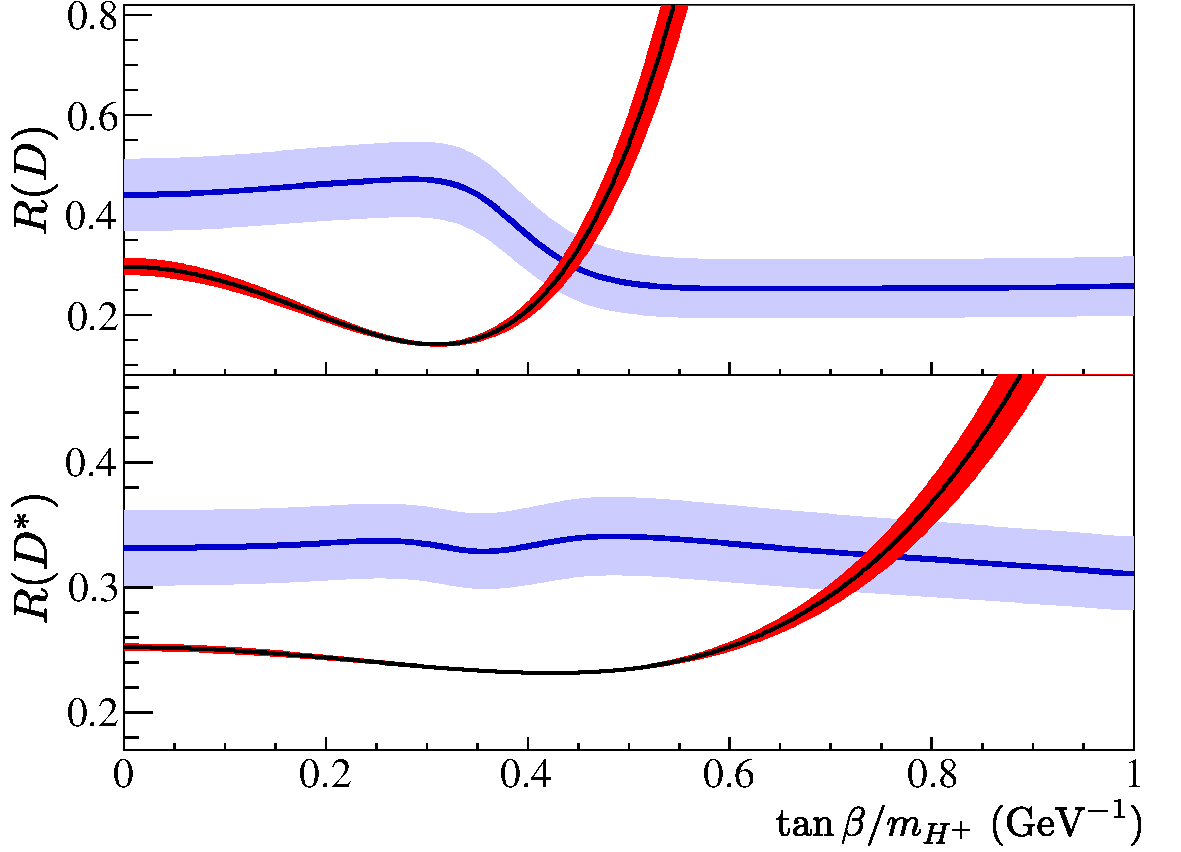
\includegraphics[width=7cm]{figures/type2_2hdm_vs_rd_rds_1205_5442.pdf}	
	}
	\only<2>{
		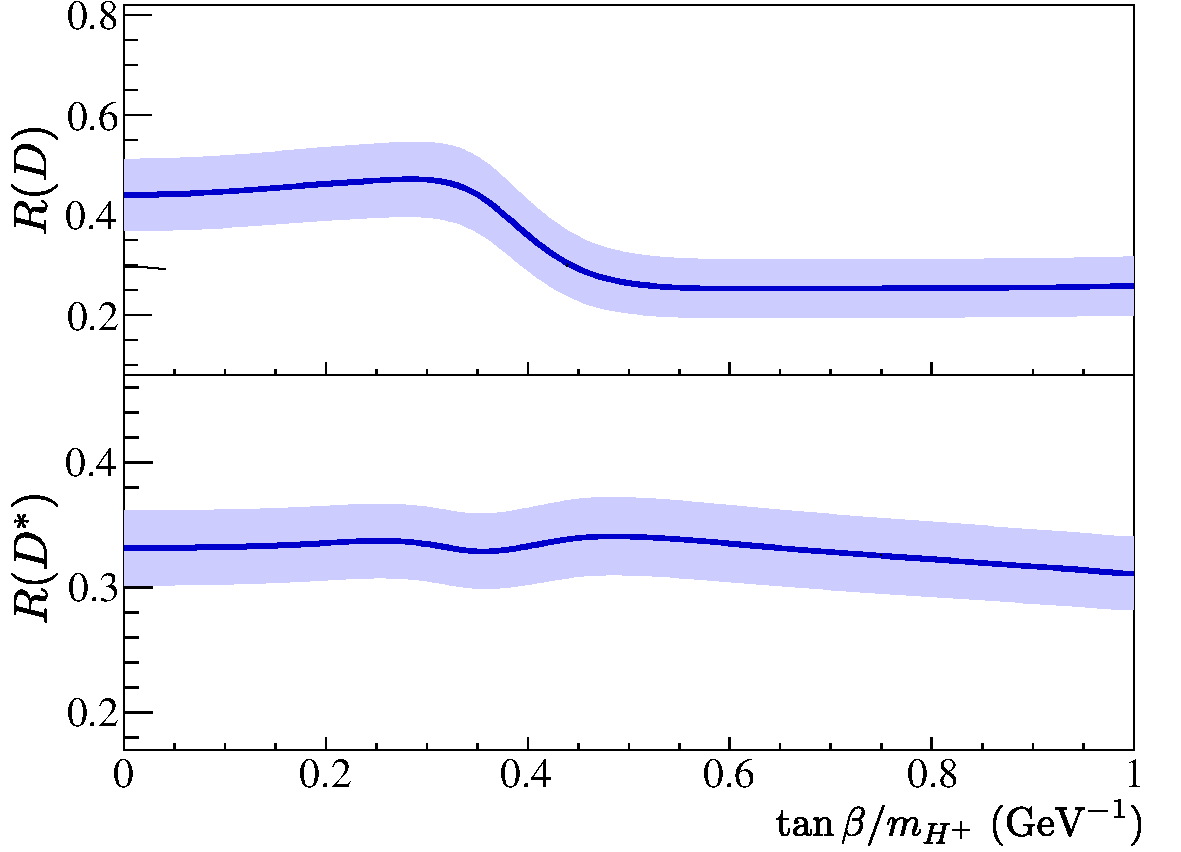
\includegraphics[width=7cm]{figures/type2_2hdm_vs_rd_rds_1205_5442_results_only.pdf}\\[1ex]
		Results obtained from a 2D fit to $m_\text{miss}^2$ and $|\vec p_\ell|$
	}
	\only<3>{
		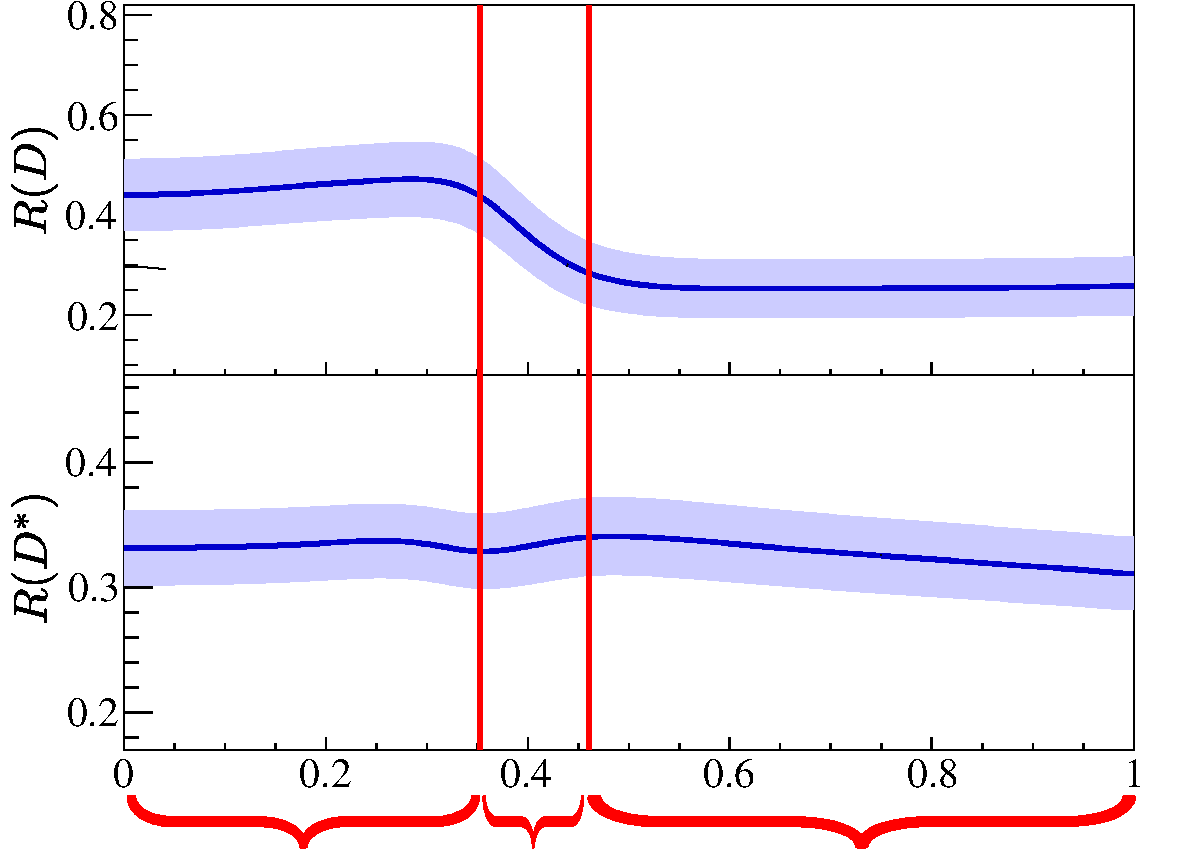
\includegraphics[width=7cm]{figures/type2_2hdm_vs_rd_rds_1205_5442_results_only_cluster.pdf}\\[1ex]
%		\begin{changemargin}{-0.25cm}{-0.25cm}
%			\small
%			kinematics of the model different $\Lra$ Would have been nice to categorize the parameter space by this behavior right away
%		\end{changemargin}
	}
	\end{center}
\end{frame}
%
\begin{frame}{Motivation III}
	\large
	\stress{Clustering of kinematic distributions}: \\[1ex]
	\badc{\textbf{Multi-dimensional parameter space}} $\longrightarrow$ \goodc{\textbf{few benchmark points}}!
	
	\bigskip
    \bigskip
	Example with 2HDMs: JHEP 1604 (2016) 126 {\footnotesize(1507.02245)}
    \begin{figure}
        \centering
    	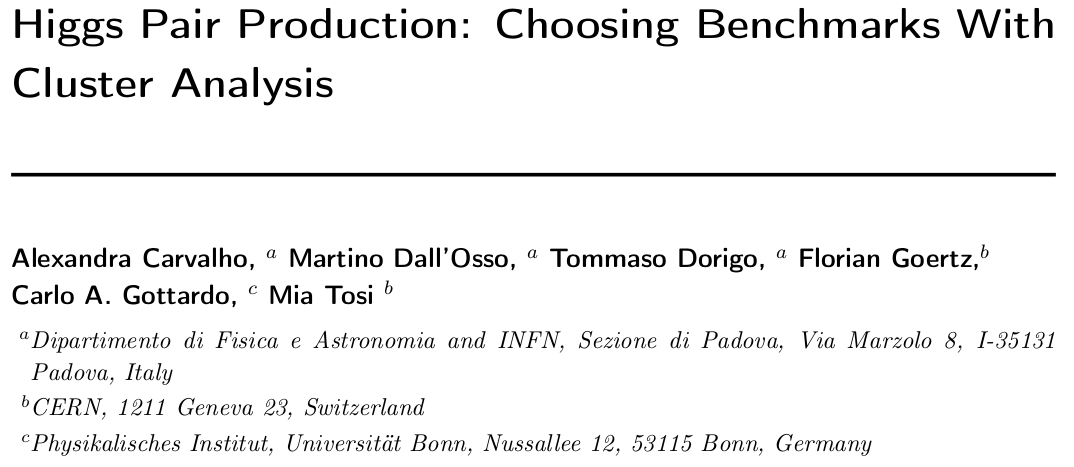
\includegraphics[height=3.3cm]{figures/scrot/2hdm_paper.png}
    \end{figure}
    
%	\bigskip
%	More general use case:\\
%	Cluster \stress{kinematic distributions} in space of \stress{Wilson coefficients}.
\end{frame}
%
%\begin{frame}{Clustering of $B\lra D^{(*)} l \nu$ kinematic shapes}
%	\textbf{Team:}
%	\begin{itemize}
%		\item Original idea/kickoff/implementation of distributions: \mauthor{Alejandro Celis} \\
%		(left in November 2018) 
%		\item Open development on \url{https://github.com/RD-clustering/B_decays_clustering/}
%		\item Also on board: \mauthor{Jason Aebischer}
%	\end{itemize}
%	\textbf{Problem:} Phenomenology of NP models depends on free parameters influencing the shape of kinematic distributions $\Lra$
%	\begin{itemize}
%		\item Difficult to present exclusion limits
%		\item An issue for analyses that need to make assumptions on kinematic distributions to extract features of interest (but still want to publish their results in a very general way)
%	\end{itemize}
%	\textbf{Solution:}
%	\begin{itemize}
%		\item Cluster NP parameter space based on a metric quantifying similarity of the result kinematic distributions
%		\item Choose NP benchmark point representing each cluster cluster
%		\item Report exclusion limits and measurements for each benchmark point
%	\end{itemize}
%\end{frame}
%%
%%
%\begin{frame}
%	\textbf{Examples:}
%	\begin{itemize}
%		\item For 2HDMs: \reference{https://arxiv.org/abs/1507.02245}{1507.02245} (used by \mauthor{ATLAS} and \mauthor{CMS})
%		\item Example of the dependency of result based on hypothesis (\mauthor{BaBar}):\\
%		
%		\medskip
%		{\centering
%			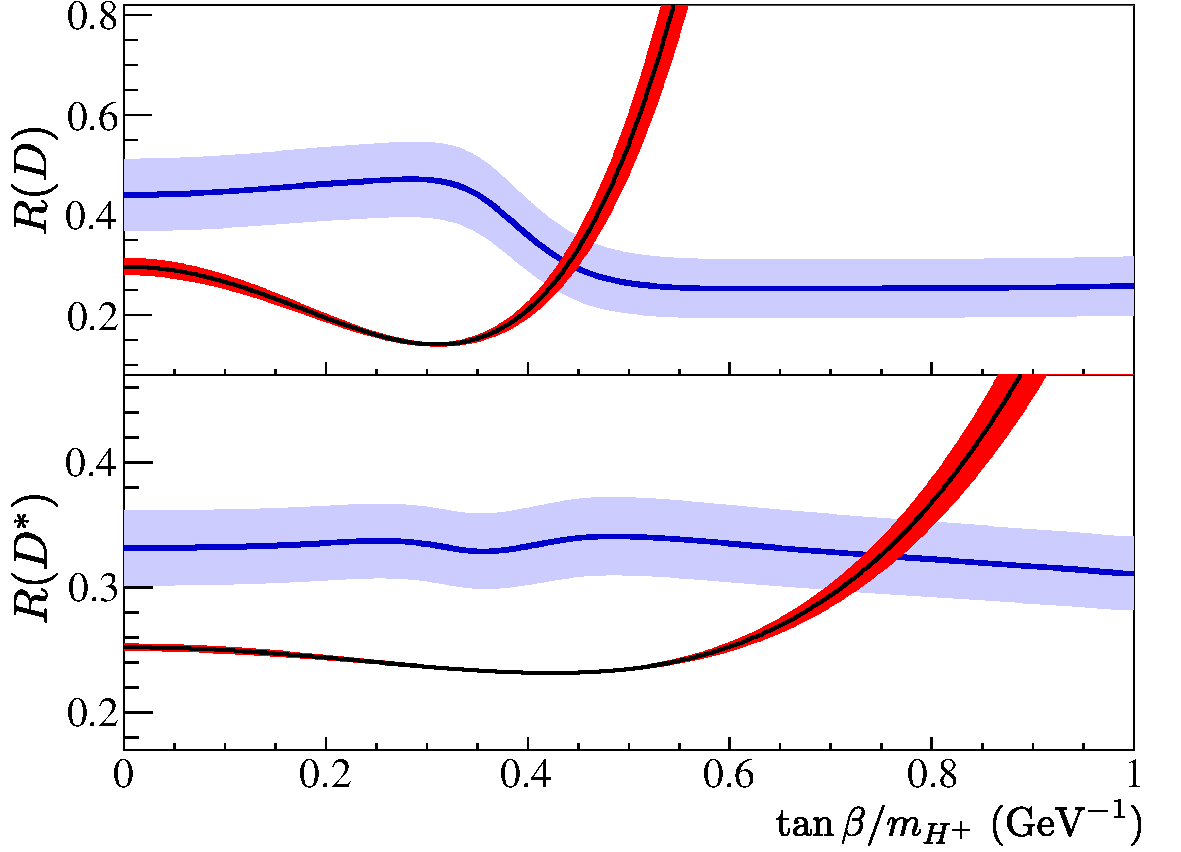
\includegraphics[width=8cm]{figures/type2_2hdm_vs_rd_rds_1205_5442.pdf}	
%			\par
%		}
%	\end{itemize}
%\end{frame}